\section{Functions and Limits}

\subsection{Functions}

\begin{paracol}{2}

\begin{tikzpicture}
\node [rounded-box] (box){\begin{minipage}{0.45\textwidth}
    A curve in the $xy$-plane is the graph of a function of $x$ if and only if no vertical line intersects the curve more than once.
\end{minipage}};
\node[rounded-box-title, left=10pt] at (box.north east) {The Vertical Line Test};
\end{tikzpicture}

\begin{tikzpicture}
\node [rounded-box] (box){\begin{minipage}{0.45\textwidth}
    A function $f$ is called \textbf{increasing} on an interval $I$ if

    $$f(x_1) < f(x_2) \text{ for all } x_1 < x_2 \text{ in } I$$
\end{minipage}};
\node[rounded-box-title, left=10pt] at (box.north east) {Definition};
\end{tikzpicture}

\begin{tikzpicture}
\node [rounded-box] (box){\begin{minipage}{0.45\textwidth}
    A function $f$ is called \textbf{decreasing} on an interval $I$ if

    $$f(x_1) > f(x_2) \text{ for all } x_1 > x_2 \text{ in } I$$
\end{minipage}};
\node[rounded-box-title, left=10pt] at (box.north east) {Definition};
\end{tikzpicture}

\switchcolumn

\begin{tikzpicture}
\node [rounded-box] (box){\begin{minipage}{0.45\textwidth}
    A function $f$ is called \textbf{even} if $f(-x) = f(x)$.
\end{minipage}};
\node[rounded-box-title, left=10pt] at (box.north east) {Definition};
\end{tikzpicture}

\begin{tikzpicture}
\node [rounded-box] (box){\begin{minipage}{0.45\textwidth}
    A function $f$ is called \textbf{odd} if $f(-x) = -f(x)$.
\end{minipage}};
\node[rounded-box-title, left=10pt] at (box.north east) {Definition};
\end{tikzpicture}

\begin{figure}
    \centering
    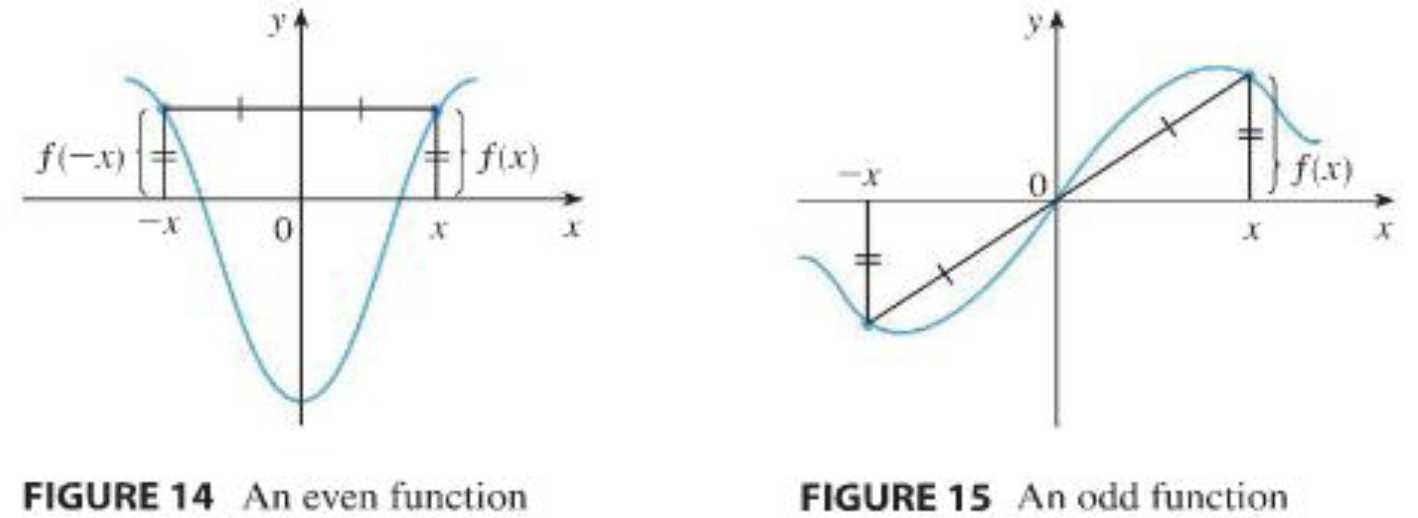
\includegraphics[width=0.95\linewidth]{even-odd-functions.png}
\end{figure}

\switchcolumn

\begin{tikzpicture}
\node [rounded-box] (box){\begin{minipage}{0.45\textwidth}
    Suppose $c > 0$. \\

    \begin{itemize}
        \item $y = f(x) + c$ shifts the graph $c$ units upward.
        \item $y = f(x) - c$ shifts the graph $c$ units downward. \\

        \item $y = f(x + c)$ shifts the graph $c$ units to the left.
        \item $y = f(x - c)$ shifts the graph $c$ units to the right.
    \end{itemize}
\end{minipage}};
\node[rounded-box-title, left=10pt] at (box.north east) {Shifts};
\end{tikzpicture}

\switchcolumn

\begin{tikzpicture}
\node [rounded-box] (box){\begin{minipage}{0.45\textwidth}
    Suppose $c > 1$. \\

    \begin{itemize}
        \item $y = - f(x)$ reflects the graph about the $x$-axis. \\

        \item $y = f(-x)$ reflects the graph about the $y$-axis.
    \end{itemize}
\end{minipage}};
\node[rounded-box-title, left=10pt] at (box.north east) {Reflections};
\end{tikzpicture}

\switchcolumn

\begin{tikzpicture}
\node [rounded-box] (box){\begin{minipage}{0.45\textwidth}
    Suppose $c > 1$.

    \begin{itemize}
        \item $y = c f(x)$ stretches the graph vertically by a factor of $c$.

        \item $y = f(x / c)$ stretches the graph horizontally by a factor of $c$.
    \end{itemize}
\end{minipage}};
\node[rounded-box-title, left=10pt] at (box.north east) {Stretches};
\end{tikzpicture}

\switchcolumn

\begin{tikzpicture}
\node [rounded-box] (box){\begin{minipage}{0.45\textwidth}
    Suppose $c > 1$. \\

    \begin{itemize}
        \item $y = \frac{1}{c} f(x)$ shrinks the graph vertically by a factor of $c$. \\

        \item $y = f(c x)$ shrinks the graph horizontally by a factor of $c$.
    \end{itemize}
\end{minipage}};
\node[rounded-box-title, left=10pt] at (box.north east) {Shrinkages};
\end{tikzpicture}

\end{paracol}

\subsection{Limits}

\begin{paracol}{2}

\begin{tikzpicture}
\node [rounded-box] (box){\begin{minipage}{0.45\textwidth}
    Suppose that $c$ is a constant and the limits $\lim_{x \rightarrow a} f(x)$ and $\lim_{x \rightarrow a} g(x)$ exist. Then \\

    \begin{enumerate}
        \item $\lim_{x \rightarrow a} [f(x) + g(x)] = \lim_{x \rightarrow a} f(x) + \lim_{x \rightarrow a} g(x)$

        \item $\lim_{x \rightarrow a} [f(x) - g(x)] = \lim_{x \rightarrow a} f(x) - \lim_{x \rightarrow a} g(x)$ \\

        \item $\lim_{x \rightarrow a} [c f(x)] = c \lim_{x \rightarrow a} f(x)$ \\

        \item $\lim_{x \rightarrow a} [f(x) g(x)] = \lim_{x \rightarrow a} f(x) \cdot \lim_{x \rightarrow a} g(x)$ \\

        \item $\lim_{x \rightarrow a} \frac{f(x)}{g(x)} = \frac{\lim_{x \rightarrow a} f(x)}{\lim_{x \rightarrow a} g(x)}$ if $\lim_{x \rightarrow a} g(x) \neq 0$ \\

        \item $\lim_{x \rightarrow a} [f(x)]^n = \Big[ \lim_{x \rightarrow a} f(x) \Big]^n$ if $n$ is a positive integer \\

        \item $\lim_{x \rightarrow a} c = c$

        \item $\lim_{x \rightarrow a} x = a$ \\

        \item $\lim_{x \rightarrow a} x^n = a^n$ if $n$ is a positive integer \\

        \item $\lim_{x \rightarrow a} \sqrt[n]{x} = \sqrt[n]{a}$ if $n$ is a positive integer \\

        \item $\lim_{x \rightarrow a} \sqrt[n]{f(x)} = \sqrt[n]{\lim_{x \rightarrow a} f(x)}$ if $n$ is a positive integer and $\lim_{x \rightarrow a} f(x) > 0$
    \end{enumerate}
\end{minipage}};
\node[rounded-box-title, left=10pt] at (box.north east) {Limit Laws};
\end{tikzpicture}

\switchcolumn

\begin{tikzpicture}
\node [rounded-box] (box){\begin{minipage}{0.45\textwidth}
    If $f$ is a polynomial or a rational function and $a$ is in the domain of $f$, then

    $$\lim_{x \rightarrow a} f(x) = f(a)$$
\end{minipage}};
\node[rounded-box-title, left=10pt] at (box.north east) {Direct Substitution Property};
\end{tikzpicture}

\begin{tikzpicture}
\node [rounded-box] (box){\begin{minipage}{0.45\textwidth}
    $$\lim_{x \rightarrow a} f(x) = L \text{ if and only if } \lim_{x \rightarrow a^-} f(x) = \lim_{x \rightarrow a^+} f(x) = L$$
\end{minipage}};
\node[rounded-box-title, left=10pt] at (box.north east) {Theorem};
\end{tikzpicture}

\begin{tikzpicture}
\node [rounded-box] (box){\begin{minipage}{0.45\textwidth}
    If $f(x) \leq g(x)$ when $x$ is near $a$ (except possibly at $a$) and the limits of $f$ and $g$ both exist as $x$ approaches $a$, then

    $$\lim_{x \rightarrow a} f(x) \leq \lim_{x \rightarrow a} g(x)$$
\end{minipage}};
\node[rounded-box-title, left=10pt] at (box.north east) {Theorem};
\end{tikzpicture}

\begin{tikzpicture}
\node [rounded-box] (box){\begin{minipage}{0.45\textwidth}
    If $f(x) \leq f(x) \leq h(x)$ when $x$ is near $a$ (except possibly at $a$) and

    $$\lim_{x \rightarrow a} f(x) = \lim_{x \rightarrow a} h(x) = L \text{ then } \lim_{x \rightarrow a} g(x) = L$$
\end{minipage}};
\node[rounded-box-title, left=10pt] at (box.north east) {The Squeeze Theorem};
\end{tikzpicture}

\end{paracol}

\subsection{Continuity}

\begin{paracol}{2}

\begin{tikzpicture}
\node [rounded-box] (box){\begin{minipage}{0.45\textwidth}
    A function $f$ is \textbf{continuous} at a number $a$ if

    $$\lim_{x \rightarrow a} f(x) = f(a)$$
\end{minipage}};
\node[rounded-box-title, left=10pt] at (box.north east) {Definition};
\end{tikzpicture}

\begin{tikzpicture}
\node [rounded-box] (box){\begin{minipage}{0.45\textwidth}
    A function $f$ is \textbf{continuous from the right} at $a$ if

    $$\lim_{x \rightarrow a^+} f(x) = f(a)$$

    A function $f$ is \textbf{continuous from the left} at $a$ if

    $$\lim_{x \rightarrow a^-} f(x) = f(a)$$
\end{minipage}};
\node[rounded-box-title, left=10pt] at (box.north east) {Definition};
\end{tikzpicture}

\begin{tikzpicture}
\node [rounded-box] (box){\begin{minipage}{0.45\textwidth}
    A function $f$ is \textbf{continuous on an interval} it is continuous at every number in the interval.
\end{minipage}};
\node[rounded-box-title, left=10pt] at (box.north east) {Theorem};
\end{tikzpicture}

\begin{tikzpicture}
\node [rounded-box] (box){\begin{minipage}{0.45\textwidth}
    If $f$ and $g$ are continuous at $a$, and $c$ is a constant, then the following functions are also continuous at $a$:

    $$f + g \qquad f - g \qquad cf \qquad fg \qquad \frac{f}{g} \text{ if } g(a) \neq 0$$
\end{minipage}};
\node[rounded-box-title, left=10pt] at (box.north east) {Theorem};
\end{tikzpicture}

\switchcolumn

\begin{tikzpicture}
\node [rounded-box] (box){\begin{minipage}{0.45\textwidth}
    The following types of functions are continuous at every number in their domains:

    \begin{itemize}
        \item Polynomials.
        \item Rational functions.
        \item Root functions.
        \item Trigonometric functions.
    \end{itemize}
\end{minipage}};
\node[rounded-box-title, left=10pt] at (box.north east) {Theorem};
\end{tikzpicture}

\begin{tikzpicture}
\node [rounded-box] (box){\begin{minipage}{0.45\textwidth}
    If $f$ is continuous at $b$ and $\lim_{x \rightarrow a} g(x) = b$, then

    $\lim_{x \rightarrow a} f(g(x)) = f\big( \lim_{x \rightarrow a} g(x) \big) = f(b)$
\end{minipage}};
\node[rounded-box-title, left=10pt] at (box.north east) {Theorem};
\end{tikzpicture}

\begin{tikzpicture}
\node [rounded-box] (box){\begin{minipage}{0.45\textwidth}
    If $g$ is continuous at $a$ and $f$ is continuous at $g(a)$, then composite function $f \circ g$ given by $(f \circ g)(x) = f(g(x))$ is continuous at $a$.
\end{minipage}};
\node[rounded-box-title, left=10pt] at (box.north east) {Theorem};
\end{tikzpicture}

\begin{tikzpicture}
\node [rounded-box] (box){\begin{minipage}{0.45\textwidth}
    Suppose that $f$ is continuous on the closed interval $[a, b]$ and let $N$ be any number between $f(a)$ and $f(b)$, where $f(a) \neq f(b)$. Then there exists a number $c$ in $(a, b)$ such that $f(c) = N$.
\end{minipage}};
\node[rounded-box-title, left=10pt] at (box.north east) {The Intermediate Value Theorem};
\end{tikzpicture}

That is, a continuous function takes on every intermediate value between the function values $f(a)$ and $f(b)$ at least once.

\end{paracol}

\subsection{Inverse Functions}

\begin{paracol}{2}

\begin{tikzpicture}
\node [rounded-box] (box){\begin{minipage}{0.45\textwidth}
    A function $f$ is called a \textbf{one-to-one function} if it never takes on the same value twice; that is,

    \vspace{5pt}

    $$f(x_1) \neq f(x_2) \text{ for all } x_1 \neq x_2$$

    \vspace{2.5pt}
\end{minipage}};
\node[rounded-box-title, left=10pt] at (box.north east) {Definition};
\end{tikzpicture}

\begin{tikzpicture}
\node [rounded-box] (box){\begin{minipage}{0.45\textwidth}
    A function is one-to-one if and only if no horizontal line intersects its graph more than once.
\end{minipage}};
\node[rounded-box-title, left=10pt] at (box.north east) {Horizontal Line Test};
\end{tikzpicture}

\begin{tikzpicture}
\node [rounded-box] (box){\begin{minipage}{0.975\textwidth}
    Let $f$ be a one-to-one function with domain $A$ and range $B$. Then its \textbf{inverse function} $f^{-1}$ has domain $B$ and range $A$ and is defined by

    $$f^{-1}(y) = x \quad \iff \quad f(x) = y$$

    for any $y$ in $B$.
\end{minipage}};
\node[rounded-box-title, left=10pt] at (box.north east) {Definition};
\end{tikzpicture}

\switchcolumn

\begin{tikzpicture}
\node [rounded-box] (box){\begin{minipage}{0.45\textwidth}
    If $f$ is a one-to-one continuous function defined on an interval, then its inverse function is also continuous.
\end{minipage}};
\node[rounded-box-title, left=10pt] at (box.north east) {Theorem};
\end{tikzpicture}

\begin{tikzpicture}
\node [rounded-box] (box){\begin{minipage}{0.45\textwidth}
    If $f$ is a one-to-one differentiable function with inverse function $f^{-1}$ and $f'(f^{-1}(a)) \neq 0$, then the inverse function is differentiable at $a$ and

    \vspace{-5pt}

    $$(f^{-1})'(a) = \frac{1}{f'(f^-1(a))}$$
\end{minipage}};
\node[rounded-box-title, left=10pt] at (box.north east) {Theorem};
\end{tikzpicture}

\end{paracol}

\subsection{Asymptotes}

\begin{paracol}{2}

\begin{tikzpicture}
\node [rounded-box] (box){\begin{minipage}{0.45\textwidth}
    \textbf{Infinite Limits}:
    
    The line $x = a$ is called a \textbf{vertical asymptote} of the curve $y = f(x)$ if at least one of the following is true:

    \vspace{-10pt}

    $$\lim_{x \rightarrow a^-} f(x) = \infty \qquad \lim_{x \rightarrow a^+} f(x) = \infty \qquad \lim_{x \rightarrow a} f(x) = \infty$$

    \vspace{-20pt}

    $$\lim_{x \rightarrow a^-} f(x) = -\infty \quad \lim_{x \rightarrow a^+} f(x) = -\infty \quad \lim_{x \rightarrow a} f(x) = -\infty$$
\end{minipage}};
\node[rounded-box-title, left=10pt] at (box.north east) {Definition};
\end{tikzpicture}

\switchcolumn

\begin{tikzpicture}
\node [rounded-box] (box){\begin{minipage}{0.45\textwidth}
    \textbf{Limits at Infinity}: \\
    
    The line $y = L$ is called a \textbf{horizontal asymptote} of the curve $y = f(x)$ if either

    \vspace{10pt}

    $$\lim_{x \rightarrow \infty} f(x) = L \qquad \text{or} \qquad \lim_{x \rightarrow -\infty} f(x) = L$$
\end{minipage}};
\node[rounded-box-title, left=10pt] at (box.north east) {Definition};
\end{tikzpicture}

\end{paracol}

The line $y = mx + b$ is called a \textbf{slant asymptote} if $\lim_{x \rightarrow \pm \infty} f(x) - (mx + b) = 0$.

\subsection{Indeterminate Forms and l'Hospital's Rule}

\begin{paracol}{2}

\begin{tikzpicture}
\node [rounded-box] (box){\begin{minipage}{0.45\textwidth}
    \textbf{Indeterminate Products}:

    \vspace{-2.5pt}

    $$fg = \frac{f}{1 / g} \qquad \text{or} \qquad fg = \frac{g}{1 / g}$$
\end{minipage}};
\node[rounded-box-title, left=10pt] at (box.north east) {Definition};
\end{tikzpicture}

\begin{tikzpicture}
\node [rounded-box] (box){\begin{minipage}{0.45\textwidth}
    \textbf{Indeterminate Differences}: If $\lim_{x \rightarrow a} f(x) = \infty$ and $\lim_{x \rightarrow a} g(x) = \infty$, then the limit $\lim_{x \rightarrow a} [f(x) - g(x)]$ is called an indeterminate form of type $\infty - \infty$.
\end{minipage}};
\node[rounded-box-title, left=10pt] at (box.north east) {Definition};
\end{tikzpicture}

\switchcolumn

\begin{tikzpicture}
\node [rounded-box] (box){\begin{minipage}{0.45\textwidth}
    \textbf{Indeterminate Powers}: $\lim_{x \rightarrow a} [f(x)]^{g(x)}$

    \begin{enumerate}
        \item Type $0^0$: $\lim_{x \rightarrow a} f(x) = 0, \lim_{x \rightarrow a} g(x) = 0$
        \item Type $\infty^0$: $\lim_{x \rightarrow a} f(x) = \infty, \lim_{x \rightarrow a} g(x) = 0$
        \item Type $1^{\pm \infty}$: $\lim_{x \rightarrow a} f(x) = 1, \lim_{x \rightarrow a} g(x) = \pm \infty$
    \end{enumerate}

    Each of these can be converted to an indeterminate product $g(x) \ln{f(x)}$ of type $0 \cdot \infty$, either by taking the natural logarithm, or by writing the function as an exponential:

    \begin{itemize}
        \item $\text{Let } y = [f(x)]^{g(x)}, \text{ then } \ln{y} = g(x) \ln{f(x)}$
        \item $[f(x)]^{g(x)} = e^{g(x) \ln{g(x)}}$
    \end{itemize}
\end{minipage}};
\node[rounded-box-title, left=10pt] at (box.north east) {Definition};
\end{tikzpicture}

\end{paracol}

\begin{tikzpicture}
\node [rounded-box] (box){\begin{minipage}{0.975\textwidth}
    Suppose $f$ and $g$ are differentiable and $g'(x) \neq 0$ near $a$ (except possibly at $a$). Suppose that we have an indeterminate form of type $0/0$ or $\infty/\infty$:

    \vspace{-10pt}

    $$\lim_{x \rightarrow a} f(x) = 0,  \lim_{x \rightarrow a} g(x) = 0 \qquad \text{or} \qquad \lim_{x \rightarrow a} f(x) = \pm \infty, \lim_{x \rightarrow a} g(x) = \pm \infty$$

    Then, if the limit on the right side exists (or is $\pm \infty$),

    $$\lim_{x \rightarrow a} \frac{f(x)}{g(x)} = \lim_{x \rightarrow a} \frac{f'(x)}{g'(x)}$$
\end{minipage}};
\node[rounded-box-title, left=10pt] at (box.north east) {L'Hospital's Rule};
\end{tikzpicture}
